\section{Experiments}
\label{sec:experiments}
We organize evaluation around four questions. Q1 tests complete systems, Q2 studies local control, and Q3 tests visual feedback. Q4 specifies the pending hardware evaluation. Q2 and Q3 use only the marked cube.

\noindent\textbf{Q1.} How do complete systems compare across objects, mappings and instruction variants?\\
\textbf{Q2.} How should the hand act during deliberation?\\
\textbf{Q3.} Does continued visual feedback help?\\
\textbf{Q4.} Does the system work on physical objects?

\subsection{Setup and reporting}
Experiments use Revo3 assets in Isaac Lab 3.0/Newton with validated contact capacities. Unless specified, each condition has two evaluation seeds and 40 scheduled trials. Physical tasks are paired within each study. Cube systems share the frozen visual pose estimator, goal bank, latent student, 0.16-radian tolerance and measured-pose stopping. Other objects use separate students and noisy simulator pose; REVEAL additionally uses calibrated completion correction. Bare VLM baselines omit the added control actors and use a fixed unreadable-view schedule, while REVEAL adapts its inspection. REVEAL denotes the complete deployed system. Natural model latency and these backend differences are part of the complete-system comparison.

The latest cube release replaces only its waiting actor. Q1 and Q3 rates use common service-eligible slots across compared methods; Q2 reports all 120 outcomes per method. Q1 and Q2 use distinct evaluation cohorts: Q1 measures complete systems across mappings, whereas Q2 isolates pending-request control on the cube. Their absolute rates are not matched estimates; controller gains are computed within Q2. The three-seed Q2 table is descriptive. Paired tests and any multiplicity corrections are specified separately for each study in the supplement.

\subsection{Q1: Systems across objects and mappings}
We compare original and changed semantic mappings across six object-specific releases. Historical native-image cohorts remain separate in the supplement; their REVEAL--fine-tuned differences are unresolved (cube $p=0.267$, die $p=0.4545$).

\begin{table*}[t]
\centering\scriptsize
\setlength{\tabcolsep}{3pt}
\begin{tabular}{llrrrrrr}
\toprule
Object & Perception & \multicolumn{3}{c}{Original mapping} & \multicolumn{3}{c}{Changed mapping}\\
\cmidrule(lr){3-5}\cmidrule(lr){6-8}
& & Rule & Fine-tuned & Full Astra & Rule & Fine-tuned & Full Astra\\
\midrule
Cube & RGB pose & 23/40 (57.5) & 30/40 (75.0) & 32/40 (80.0) & 23/40 (57.5) & 16/40 (40.0) & 32/40 (80.0)\\
Die & Noisy pose & 13/40 (32.5) & 23/40 (57.5) & 28/40 (70.0) & 1/40 (2.5) & 0/40 (0.0) & 26/40 (65.0)\\
Duck & Noisy pose & 15/38 (39.5) & 14/38 (36.8) & 25/38 (65.8) & 9/40 (22.5) & 2/40 (5.0) & 24/40 (60.0)\\
Hedgehog & Noisy pose & 17/39 (43.6) & 13/39 (33.3) & 28/39 (71.8) & 10/40 (25.0) & 2/40 (5.0) & 32/40 (80.0)\\
Pig & Noisy pose & 21/40 (52.5) & 16/40 (40.0) & 37/40 (92.5) & 15/40 (37.5) & 3/40 (7.5) & 33/40 (82.5)\\
Milk carton & Noisy pose & 13/40 (32.5) & 9/40 (22.5) & 17/40 (42.5) & 3/40 (7.5) & 1/40 (2.5) & 11/40 (27.5)\\
\bottomrule
\end{tabular}
\caption{\textbf{Q1: system comparison across six objects and two semantic mappings.} Entries give successes / common service-eligible trials (percent), retaining 40 raw trials per cell. Fine-tuned and rule baselines omit the added control modules. Each object uses its own frozen student and adaptation. The cube uses reconstructed upper-level images and RGB pose, the die rotates its visual mesh, and the four new objects permute surface letters in native RGB with noisy simulator pose. Within each object, both mappings share physical assets and weights. These mapping cohorts are separate from the native-image release comparisons. No cross-release pooled average or zero-shot object-transfer claim is made.}
\label{tab:q1-all-objects}
\end{table*}


\paragraph{Aggregate system performance.}
Over 1,440 scheduled trials, equal-object mean success is \QOneOriginalSuccess\% on original mappings and \QOneChangedSuccess\% on changed mappings. The strongest baseline means are \QOneOriginalBaseline\% (fine-tuning) and \QOneChangedBaseline\% (rules), yielding gains of \QOneOriginalGain{} and \QOneChangedGain{} percentage points. These post-hoc descriptive means weight six service-eligible object rates equally; they neither pool trials nor add a significance test.


\paragraph{Four additional objects.}
Duck, hedgehog, pig and milk carton contribute 960 trials across two mappings. REVEAL has the highest observed rate in each cell (Table~\ref{tab:q1-all-objects}); these are object-specific systems, not common-policy transfer. Three historical service failures are excluded symmetrically. Milk-carton REVEAL drops in 15/40 original and 20/40 changed-mapping trials, so higher completion does not imply stable grasping. Reset and sensitivity audits are in the supplement.

\paragraph{Visual-semantic intervention.}
Only the upper image changes; predictor input and lighting remain fixed. Identity, cyclic letter--color permutation and masking use 40 matched states per method, all with reconstructed face images. REVEAL retains 32/40 successes after permutation; fine-tuning falls from 30/40 to 16/40 (Holm $p=0.0130$, six contrasts); rules remain at 23/40. Masking yields 0/39, 3/40 and 0/40, respectively (full supplement table). Nine of eleven fine-tuned wrong bindings after permutation select the old association, consistent with learned shortcuts but not an exclusive memorization mechanism. One permutation does not establish broad generalization or equivalence.

\paragraph{Dice layout transfer.}
A separate 240-trial study rotates only the native visual mesh, preserving collision, inertia and the prompt distinguishing printed counts from motor-skill IDs. Table~\ref{tab:q1-all-objects} reports 40 matched trials per cell, with no exclusions. Permuted-layout REVEAL contrasts give exploratory paired $p=2.98\times10^{-8}$ against fine-tuning and $p=5.96\times10^{-8}$ against rules; its layout contrast ($p=0.688$) does not establish equivalence. REVEAL also receives probes, history and noisy feedback, so this supports system-level transfer, not isolated model superiority.

\paragraph{Language and wording coverage.}
Three object-specific cohorts test English/Chinese standard and rewritten instructions: three evaluation seeds, 60 scheduled trials per cell, 2,160 total. Table~\ref{tab:language-objects} uses common service-eligible slots; weights, mappings and scoring remain fixed, without Chinese retraining. The rule baseline also localizes its task/output instructions, so this tests deployed-system coverage. Rates are conditional on service availability; the supplement retains raw outcomes.

REVEAL reaches 67.8--76.7\% on duck and 73.3--76.7\% on hedgehog, exceeding fine-tuning in all eight conditions (Holm-adjusted paired $p\leq0.0258$ across 36 method contrasts). Against rules, six of eight contrasts survive correction; English-standard differences remain unresolved. On cube, REVEAL leads numerically in three conditions, while fine-tuning leads on Chinese rewriting (81.1\% versus 67.9\%); none of their four contrasts is significant (all adjusted $p=1.0$). Strict pairing sensitivity preserves these decisions. No language/wording contrast survives its separate 36-test correction; this does not establish language equivalence.

\begin{table}[t]
\centering
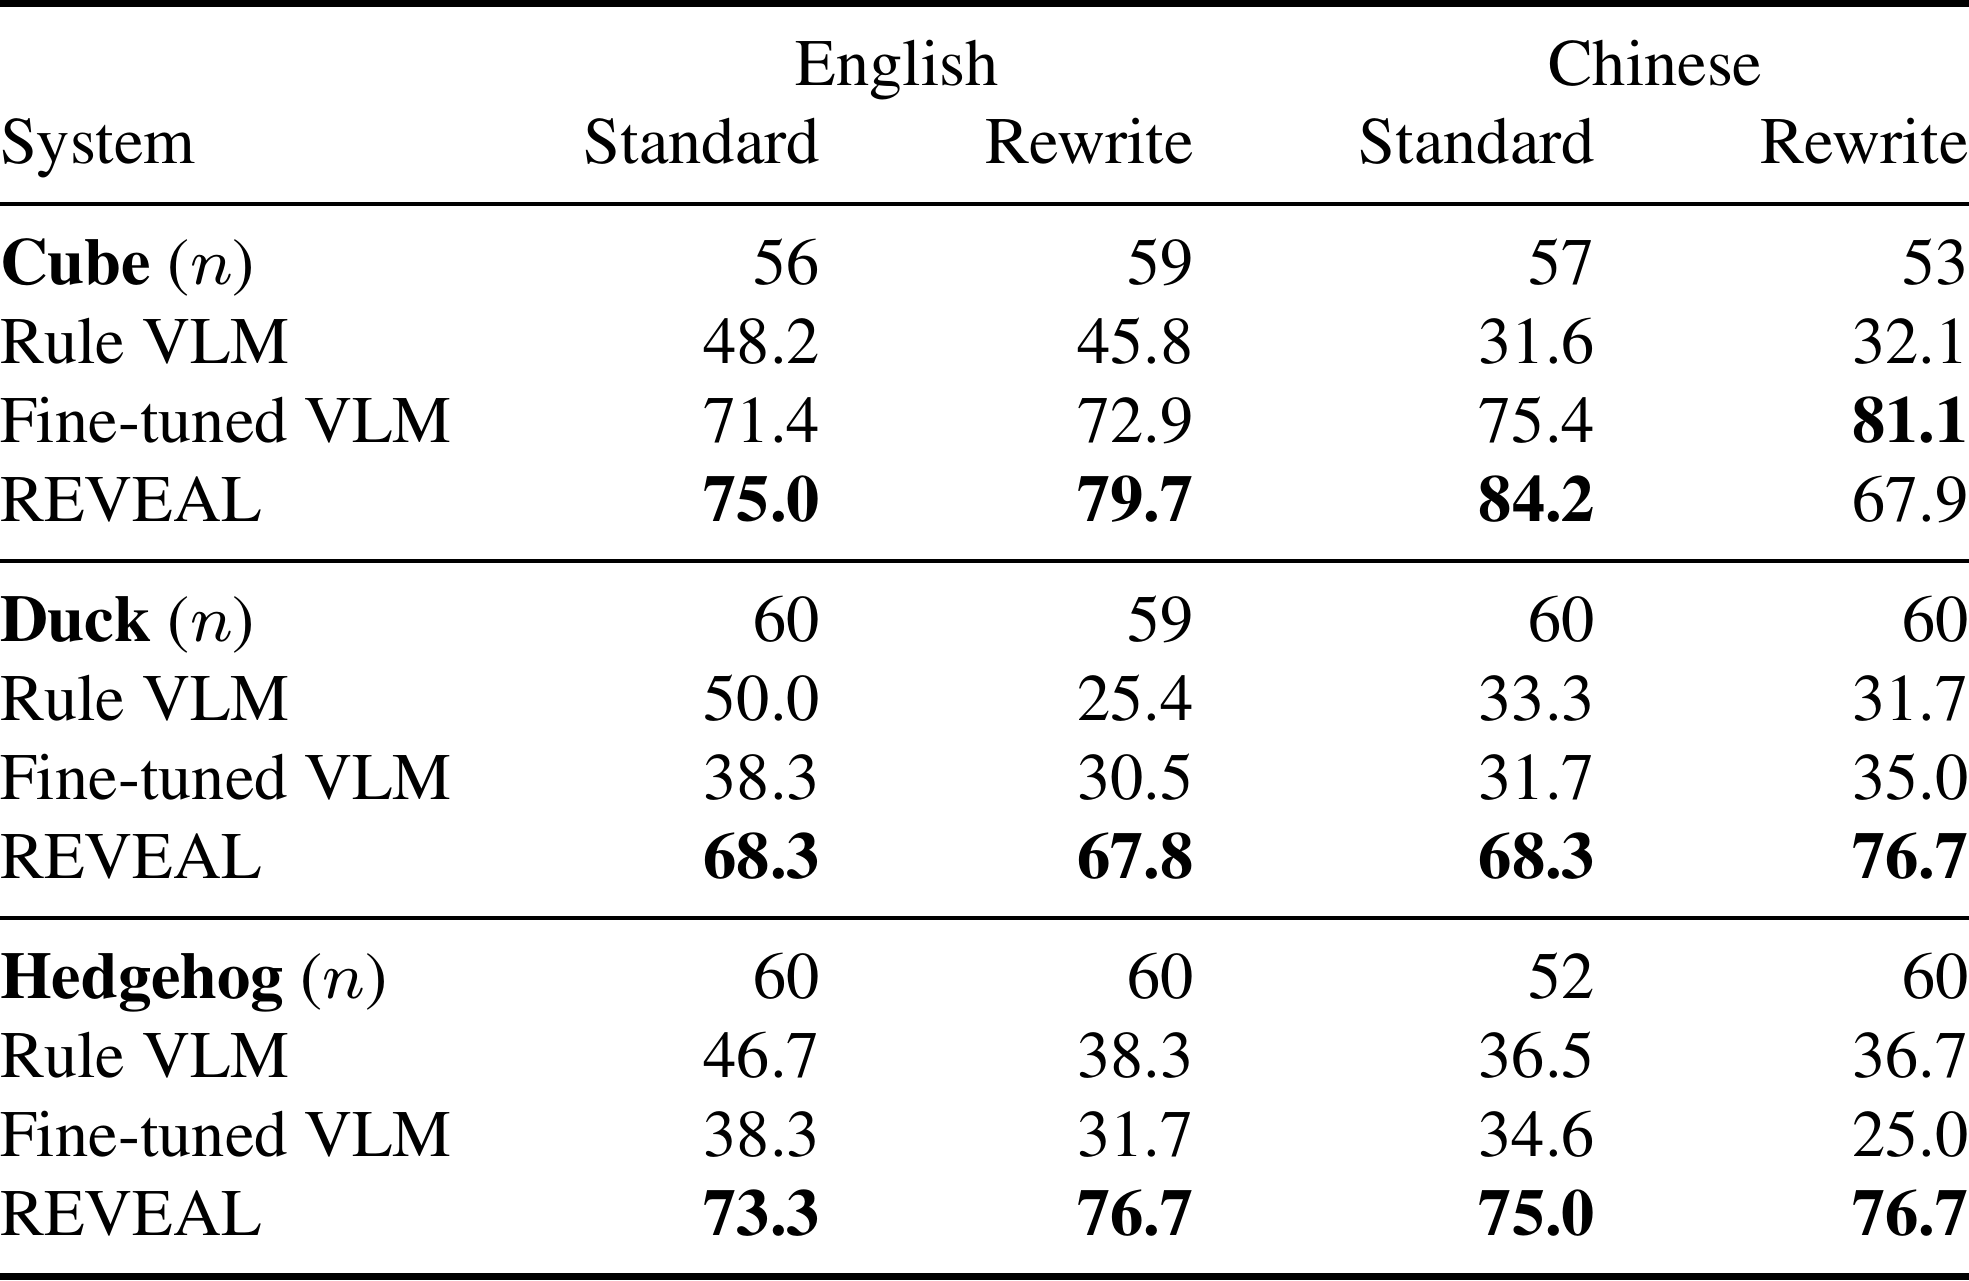
\includegraphics[width=\linewidth]{figures/language_objects.png}
\caption{\textbf{Q1: language and wording coverage.} Completion (\%) on common service-eligible trials. Methods share the listed $n$ of 60 scheduled slots. Bold denotes the highest observed rate, not significance. Raw counts and paired analyses are in the supplement.}
\label{tab:language-objects}
\end{table}


\subsection{Q2: Controller ablations on the cube}
We compare four ways of acting while a semantic request is pending: continuing the student proposal, fixed slowing with coefficient 0.15, learned slowing, and learned slowing with a bounded joint correction. The ablation changes pending-request control while retaining the same execution controller outside pending intervals. Each method is evaluated for 120 trials, with 40 trials per seed across three seeds.

\begin{table}[t]
\centering\small
\setlength{\tabcolsep}{2.5pt}
\begin{tabularx}{\linewidth}{@{}Xrrrrr@{}}
\toprule
Waiting policy & Success & \% & \shortstack{Wait\\drops} & \shortstack{Exec.\\drops} & Other\\
\midrule
Continue student & 73/120 & 60.8 & 24 & 14 & 9\\
Fixed slowing & 88/120 & 73.3 & 13 & 8 & 11\\
Learned slowing & 82/120 & 68.3 & 7 & 14 & 17\\
\textbf{Slowing + correction} & \textbf{104/120} & \textbf{86.7} & \textbf{5} & \textbf{4} & \textbf{7}\\
\bottomrule
\end{tabularx}
\caption{\textbf{Q2: controller ablation on the cube.} Each method has 120 trials across three seeds. Wait and execution drops denote failure stages; Other contains the remaining failures. Outcome counts sum to 120 in each row.}
\label{tab:waiting}
\end{table}


Slowing with joint correction achieves 104/120 successes (86.7\%), compared with 88/120 (73.3\%) for fixed slowing, a gain of 13.3 percentage points. Waiting drops decrease from 13 to five, and execution drops from eight to four. Learning the speed alone yields 82/120 successes (68.3\%), below fixed slowing. These results favor combining speed adaptation with joint correction in this evaluation; failure stages describe when a drop occurs rather than identifying its cause. Seed settings and outcome breakdowns are reported in the supplement.

\subsection{Q3: Visual feedback on the cube}
\begin{figure*}[t]
\centering
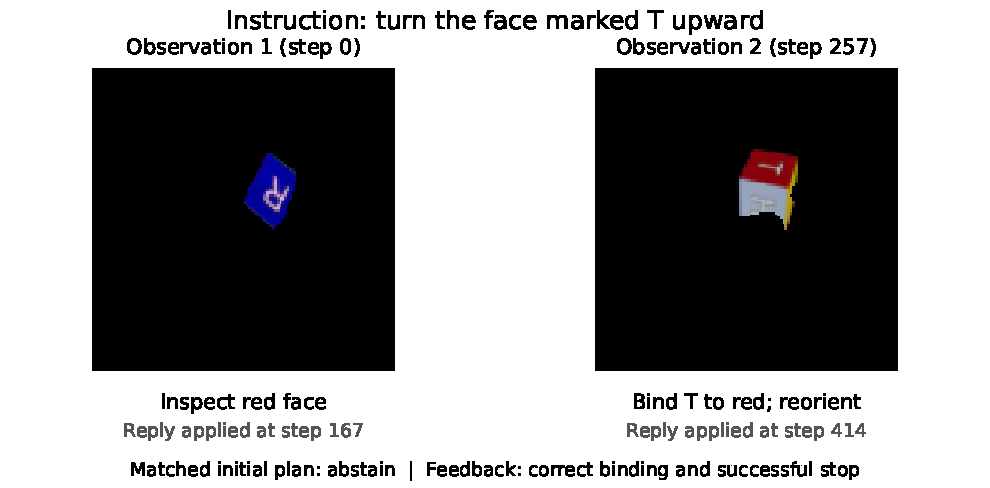
\includegraphics[width=0.86\textwidth]{figures/feedback_example.pdf}
\caption{\textbf{Recorded inspection before binding.} Unretouched model-input frames from a recorded simulated trial. The initial plan abstains; feedback reveals T, then REVEAL binds T to red and completes at step 420 (true error 0.0812 radians). Both arms start from identical state and image. This selected example illustrates evidence acquisition, not wrong-binding correction or hardware performance.}
\label{fig:recorded-search}
\end{figure*}
We test two complementary interventions in separate paired cohorts (Table~\ref{tab:q3-feedback}). Panel (a) compares complete feedback protocols; panel (b) isolates whether later images carry useful evidence under a common call cap. Their outcomes are not pooled.

\begin{table}[t]
\centering\small
\begin{tabular}{lrrrr}
\toprule
Condition & Success & \% & Drops & Calls\\
\midrule
\multicolumn{5}{l}{\textbf{(a) Continued feedback: one vs. up to six calls}}\\
\AblationFeedbackRows
\midrule
\multicolumn{5}{l}{\textbf{(b) Fresh visual evidence: same six-call cap}}\\
\ImageRefreshRows
\bottomrule
\end{tabular}
\caption{\textbf{Q3: feedback and fresh evidence on the cube.} Each panel has 40 scheduled trials per arm. (a) excludes one service-affected pair; its full-feedback arm reuses the initial 40-trial Q2 subset. (b) has no exclusions and changes only upper-agent RGB. Drops and calls are raw totals. Cohorts are separate; realized calls are not matched compute.}
\label{tab:q3-feedback}
\label{tab:feedback}
\label{tab:image-refresh}
\end{table}

\paragraph{(a) Is continued feedback useful?}
The initial-plan arm receives the first RGB observation and measured feedback, then commits to one to six bounded actions without later semantic observations. Its last non-abstain skill can continue until the common stopping gate or horizon. Full feedback permits up to six calls with updated observations and history. Both arms retain continuous student pose feedback, identical local controllers and the same stopping rule.

Success rises from 6/39 to 33/39 eligible trials: 27 pairs succeed only with feedback and none only with the initial plan (exact $p=1.49\times10^{-8}$). Raw success is 6/40 versus 34/40; an initial-plan HTTP 503 timeout is excluded symmetrically. Of 28 eligible initial-plan abstentions, 22 succeed with feedback. Among eligible feedback trials, 36 inspect, 32 first bind after inspection, and 31 successes use multiple calls. This supports evidence acquisition before binding, not correction of an executed wrong binding. Calls total 40 versus 120, so this contrast includes differing inference budgets. Zero initial-plan drops accompany frequent abstention. Figure~\ref{fig:recorded-search} shows a recorded example.

\paragraph{(b) Does the next image matter?}
Both arms retain the same six-call cap and trigger policy. Only upper-agent RGB changes: current images versus the exact first frame on every call. Numeric pose feedback, history, lower perception and control remain live. Forty pairs share initial states and first images, without exclusions.

Current images yield 32/40 successes versus 9/40 for repeated first frames. All 23 discordant pairs favor fresh images, a 57.5-point gain (exact $p=2.38\times10^{-7}$). A post-hoc audit finds correct terminal bindings in 34/40 versus 9/40 trials. Abstentions fall from 24 to two, while drops change from four to three. This pattern supports acquiring target evidence rather than a gain explained solely by fewer drops. Transport hashes verify delivered images. Actual calls, tokens and trajectories differ, so the common cap does not equalize realized compute.

\subsection{Q4: Multi-object hardware evaluation}
\paragraph{Hardware protocol.}
\TODO{Complete the multi-object physical-hand evaluation.} No hardware outcomes are available yet. The planned comparison uses REVEAL and two baselines per object, reporting completion, drops, false stops and inference cost. Calibration, resets, independent scoring and synchronized-video requirements are specified in the supplement.


\paragraph{Supporting cube perception study.}
On 6,144 rendered observations, RGB-D reaches 64.73\% pose recall versus 37.53\% for RGB at $10$~mm/$10^\circ$. Ideal masks and virtual depth limit this estimator comparison; downstream gains and physical-camera accuracy remain untested. The supplement details its protocol and occlusion analysis.
